\documentclass[11pt]{article}
\usepackage[a4paper,margin=1in]{geometry}
\usepackage[T1]{fontenc}
\usepackage[utf8]{inputenc}
\usepackage{lmodern}
\usepackage{amsmath}
\usepackage{amssymb}
\usepackage{booktabs}
\usepackage{graphicx}
\usepackage{tikz}
\usepackage{xcolor}
\usepackage{listings}
\usepackage{float}
\usepackage{longtable}
\usepackage{array}
\usepackage{caption}
\usepackage{setspace}
\usepackage{titlesec}

\onehalfspacing
\setlength{\parindent}{0pt}
\setlength{\parskip}{0.6em}

\lstdefinelanguage{TLA}{
  morekeywords={MODULE,EXTENDS,CONSTANT,CONSTANTS,VARIABLES,ASSUME,Init,Next,Spec,TypeOK,THEOREM},
  sensitive=true,
  morecomment=[l]{\\*},
  morestring=[b]"
}

\lstset{
  basicstyle=\ttfamily\small,
  keywordstyle=\color{black},
  commentstyle=\color{black},
  stringstyle=\color{black},
  breaklines=true,
  frame=single,
  columns=fullflexible
}

\title{\textbf{Weak Binary Semaphore Mutual Exclusion in TLA+}\\Final Project Report for CE356}
\author{Tianbin Wang \and Kehao Zhang}
\date{June 2026}

\newcommand{\growthlegendbox}{%
\fbox{%
\begin{tabular}{@{}c@{\hspace{0.4em}}c@{\hspace{1.2em}}c@{\hspace{0.4em}}c@{}}
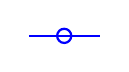
\begin{tikzpicture}[baseline=-0.6ex]
\draw[blue, thick] (0,0) -- (0.9,0);
\draw[blue, thick] (0.45,0) circle (0.09);
\end{tikzpicture}
& Baseline
&
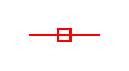
\begin{tikzpicture}[baseline=-0.6ex]
\draw[red, thick] (0,0) -- (0.9,0);
\draw[red, thick] (0.37,-0.08) rectangle (0.53,0.08);
\end{tikzpicture}
& Udding
\end{tabular}}%
}

\begin{document}
\maketitle

\begin{abstract}
We study the CE356 project on weak binary semaphores. We focus on $n$-process mutual exclusion. We use only weak binary semaphores. We use TLA+ and TLC to check correctness. We compare a simple baseline with a Udding-style protocol. We use Peterson's algorithm as background. We then explain why weak semaphores create a fairness problem. We run TLC experiments for $n=2$ through $n=7$. We also add fairness assumptions and temporal properties to the Udding model. We then check no-starvation for small instances. Our results show that both models satisfy the checked safety properties. Our results also show that the Udding model supports fairness-oriented liveness checking at small scale. We argue that this extra power comes with a much larger state space.
\end{abstract}

\section{Introduction}

The project guideline asks us to implement $n$-process mutual exclusion with only weak binary semaphores. The guideline also asks us to show correctness in TLA+. This task creates a direct tension between exclusion and fairness. A very small semaphore protocol can satisfy exclusion. A fairness-oriented protocol needs much more structure.

We follow the same direction as our midterm report. We now extend that direction into a complete final report. We compare two designs:

\begin{itemize}
  \item a simple baseline that uses a single weak binary semaphore to protect the critical section;
  \item a Udding-style protocol that introduces a staged admission discipline to better control overtaking.
\end{itemize}

We use this comparison to answer three questions. First, what can a naive weak-semaphore mutex already guarantee? Second, why is that guarantee still not enough for fairness? Third, how much extra modeling cost do we pay when we move to a fairness-oriented design?

\section{Background}

\subsection{Weak binary semaphores and fairness}

A binary semaphore takes values in $\{0,1\}$. A binary semaphore supports the usual $P$ and $V$ operations. In the weak case, the semaphore does not promise a strongly fair service rule for blocked processes. As a result, one waiting process may keep losing contention even when the whole system still makes progress.

This issue makes the project interesting. We do not only want mutual exclusion. We also want to understand how much structure a protocol needs when the primitive itself does not provide enough fairness.

\subsection{Classical mutual exclusion background: Peterson's algorithm}

Peterson's algorithm is a classical software-only mutual exclusion algorithm. We use it as conceptual background. In the two-process case, each process raises a flag and writes the shared variable \texttt{turn}:

\begin{lstlisting}
flag[i] := TRUE;
turn := j;
while flag[j] /\ turn = j do skip;
CS;
flag[i] := FALSE;
\end{lstlisting}

Peterson's algorithm is useful because it shows how shared variables can enforce mutual exclusion. However, Peterson's algorithm is not the final protocol for this project. The project requires weak binary semaphores. We therefore use Peterson's algorithm as background, not as the main experimental baseline.

\subsection{Semaphore baseline used in our experiments}

For the actual weak-semaphore baseline, we use the simplest protocol:

\begin{lstlisting}
NCS;
P(mutex);
CS;
V(mutex);
\end{lstlisting}

This baseline matches the project restriction. This baseline also shows the fairness problem very clearly. The protocol enforces exclusion, but the protocol does not stop indefinite overtaking.

\section{Why Udding's Algorithm Matters}

Udding's algorithm is directly relevant to our project. Udding designed this algorithm to address individual starvation under weak semaphores. The algorithm does not let every process race directly for the final mutex. The algorithm uses a staged pipeline. The pipeline separates outer contenders from processes that are already closer to the critical section.

The protocol we model has the following structure:

\begin{lstlisting}
P(enter); ne := ne + 1; V(enter);
P(queue); P(enter); nm := nm + 1; ne := ne - 1;
if ne > 0 then V(enter) else V(mutex);
V(queue);
P(mutex); nm := nm - 1;
CS;
if nm > 0 then V(mutex) else V(enter)
\end{lstlisting}

The role of each shared object is as follows:

\begin{itemize}
  \item \texttt{enter} controls whether new outer contenders may continue inward;
  \item \texttt{queue} serializes competition around the second \texttt{P(enter)};
  \item \texttt{mutex} controls the innermost path to the critical section;
  \item \texttt{ne} counts outer-layer contenders;
  \item \texttt{nm} counts processes waiting in the inner layer.
\end{itemize}

This design matters for fairness. The extra structure is not cosmetic. The structure prevents later arrivals from interfering arbitrarily with processes that are already deeper in the waiting pipeline. In other words, Udding already contains this fairness-oriented idea. Our TLA+ additions only make that idea explicit enough for TLC to check.

\section{TLA+ Models}

\subsection{Baseline model}

We model the baseline in TLA+ with one semaphore variable and one per-process control-state function. Each process moves through \texttt{ncs}, \texttt{trying}, \texttt{cs}, and \texttt{exit}. We check the following safety property:

\begin{lstlisting}[language=TLA]
InCS == {i \in Proc : pc[i] = "cs"}
MutualExclusion == Cardinality(InCS) <= 1
\end{lstlisting}

This model stays simple on purpose. We want this model to represent the smallest semaphore-based protocol that still solves mutual exclusion.

\subsection{Udding model}

We model the Udding protocol in TLA+ with the following variables:

\begin{itemize}
  \item \texttt{pc}
  \item \texttt{enter}
  \item \texttt{queue}
  \item \texttt{mutex}
  \item \texttt{ne}
  \item \texttt{nm}
\end{itemize}

The model breaks the protocol into small atomic actions. The model includes the outer entry phase, the queueing phase, the handoff phase, the mutex-wait phase, and the exit phase. In addition to \texttt{TypeOK} and \texttt{MutualExclusion}, we also check:

\begin{lstlisting}[language=TLA]
SplitBinary == enter + mutex \in {0, 1}
\end{lstlisting}

This invariant captures the intended split-binary-semaphore discipline between \texttt{enter} and \texttt{mutex}.

\subsection{Fairness and liveness layer}

To move beyond pure safety, we add the following definitions to the Udding model:

\begin{itemize}
  \item a per-process request predicate \texttt{Requesting(i)};
  \item a per-process critical-section predicate \texttt{InCSProc(i)};
  \item a temporal property \texttt{StarvationFree(i) == Requesting(i) \textasciitilde> InCSProc(i)};
  \item a system-level property \texttt{NoStarvation}.
\end{itemize}

We also add two fairness layers:

\begin{itemize}
  \item \texttt{ProcessFairness}, which applies weak fairness to each process step;
  \item \texttt{SemaphoreFairness}, which applies strong fairness to the key blocking acquisitions \texttt{PEnter1}, \texttt{PQueue}, \texttt{PEnter2}, and \texttt{PMutex}.
\end{itemize}

The resulting specification is:

\begin{lstlisting}[language=TLA]
FairSpec == Spec /\ ProcessFairness /\ SemaphoreFairness
\end{lstlisting}

This refinement matters. If we only use coarse process-level fairness, TLC finds a starvation counterexample. If we add fairness assumptions at the semaphore-acquisition level, TLC can check the no-starvation property for small instances.

\subsection{Code excerpts}

The baseline and Udding specifications are short enough to inspect directly. We include the full TLA+ code in the appendices. We do this to keep the report self-contained.

\section{Experimental Method}

We run TLC on both models with the following process-set parameter:

\[
Proc = \{1,2,\dots,n\}, \quad n \in \{2,3,4,5,6,7\}.
\]

For the baseline model, we check:

\begin{itemize}
  \item \texttt{TypeOK}
  \item \texttt{MutualExclusion}
\end{itemize}

For the Udding model, we check:

\begin{itemize}
  \item \texttt{TypeOK}
  \item \texttt{MutualExclusion}
  \item \texttt{SplitBinary}
\end{itemize}

For fairness-oriented liveness checking, we also prepare:

\begin{itemize}
  \item a two-process liveness configuration using \texttt{FairSpec};
  \item a three-process liveness configuration using \texttt{FairSpec};
  \item the temporal property \texttt{NoStarvation}.
\end{itemize}

We save the raw TLC output for every run. We then summarize all runs in one CSV table. We use that table for both the report tables and the plots.

\section{Experimental Results}

\subsection{Complete result table}

\begin{table}[H]
\centering
\caption{TLC results for $n=2$ through $n=7$}
\begin{tabular}{ccccccc}
\toprule
$n$ & Baseline Gen. & Baseline Dist. & Baseline Depth & Udding Gen. & Udding Dist. & Udding Depth \\
\midrule
2 & 21 & 12 & 5 & 131 & 88 & 23 \\
3 & 73 & 32 & 6 & 973 & 520 & 33 \\
4 & 225 & 80 & 7 & 6401 & 2880 & 43 \\
5 & 641 & 192 & 8 & 38961 & 15264 & 53 \\
6 & 1729 & 448 & 9 & 224257 & 78208 & 63 \\
7 & 4481 & 1024 & 10 & 1236929 & 390016 & 73 \\
\bottomrule
\end{tabular}
\end{table}

\subsection{Growth plots}

\begin{figure}[H]
\centering
\growthlegendbox

\vspace{0.8em}
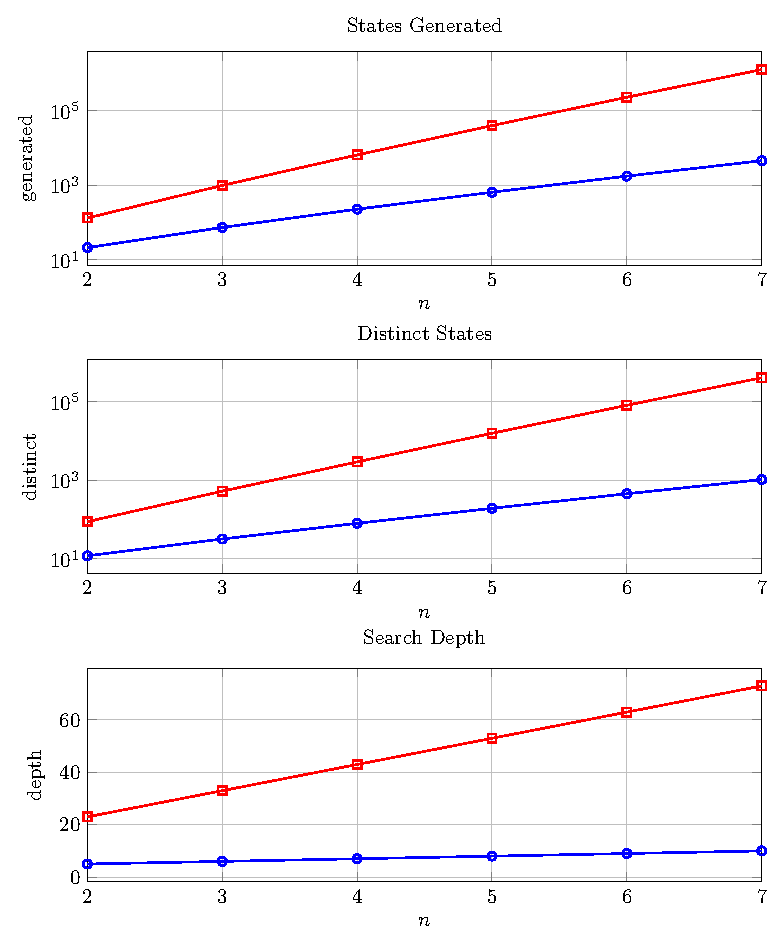
\includegraphics[width=0.88\textwidth]{results/plots/state_growth_plots.pdf}
\caption{Growth of generated states, distinct states, and search depth for the baseline and Udding models.}
\end{figure}

\begin{figure}[H]
\centering
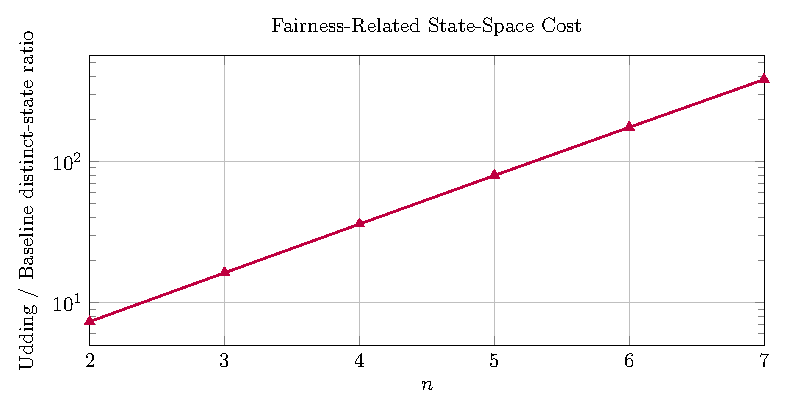
\includegraphics[width=0.72\textwidth]{results/plots/distinct_ratio_plot.pdf}
\caption{Distinct-state ratio of Udding to baseline. This ratio captures how much extra state-space cost we pay for fairness-related protocol structure.}
\end{figure}

\subsection{Fairness-oriented liveness results for Udding}

After enriching the Udding model with \texttt{FairSpec} and \texttt{NoStarvation}, we ran TLC on the following small parameter instances:

\begin{table}[H]
\centering
\caption{Liveness-oriented TLC results for Udding}
\begin{tabular}{ccccc}
\toprule
$n$ & Specification & Property & Result & Time \\
\midrule
2 & \texttt{FairSpec} & \texttt{NoStarvation} & pass & under 1 second \\
3 & \texttt{FairSpec} & \texttt{NoStarvation} & pass & about 11 seconds \\
\bottomrule
\end{tabular}
\end{table}

These results matter for the main claim of the project. The results show that the TLA+ model captures the safety discipline of Udding's protocol. The results also show that the model captures its intended anti-starvation behavior under explicit fairness assumptions.

\section{Comparison and Analysis}

\subsection{Both models satisfy the checked safety properties}

For all tested values of $n$ from 2 through 7, both models pass TLC with no invariant violation. This result shows that both protocols satisfy mutual exclusion in the parameter range that we explored.

\subsection{The real difference is fairness-related structure}

The baseline is enough if we only ask for exclusion. The baseline is small, direct, and easy to verify. However, the baseline does not regulate how contenders are admitted. Under weak fairness, this means a waiting process can still be overtaken again and again.

The Udding protocol is different in a fundamental way. The protocol adds a staged admission structure. The protocol separates outer waiting, queue serialization, and inner waiting. This structure makes the model fairness-conscious. The larger state space is therefore not accidental overhead. The larger state space reflects extra commitments about how the protocol organizes contention.

This interpretation is now supported in two ways:

\begin{itemize}
  \item by safety-oriented parameter sweeps for $n=2$ through $n=7$;
  \item by liveness-oriented \texttt{NoStarvation} checks for $n=2$ and $n=3$ under explicit fairness assumptions.
\end{itemize}

\subsection{State-space cost of fairness}

The clearest quantitative result is the ratio between the distinct-state counts of the Udding and baseline models:

\begin{table}[H]
\centering
\caption{Distinct-state ratio of Udding to baseline}
\begin{tabular}{cccc}
\toprule
$n$ & Baseline Distinct & Udding Distinct & Ratio \\
\midrule
2 & 12 & 88 & 7.33x \\
3 & 32 & 520 & 16.25x \\
4 & 80 & 2880 & 36.00x \\
5 & 192 & 15264 & 79.50x \\
6 & 448 & 78208 & 174.57x \\
7 & 1024 & 390016 & 380.88x \\
\bottomrule
\end{tabular}
\end{table}

This trend supports our main interpretation. As we increase the number of processes, the fairness-aware admission discipline of Udding becomes much more expensive to model and verify than the simple baseline.

\subsection{Peterson, baseline, and Udding in perspective}

We can now place the three ideas in a useful hierarchy:

\begin{itemize}
  \item Peterson's algorithm gives us classical mutual exclusion intuition.
  \item The single-\texttt{mutex} semaphore baseline gives us the correct weak-semaphore comparison point.
  \item Udding's algorithm gives us a fairness-oriented semaphore design for the actual project setting.
\end{itemize}

This layered presentation is useful because it shows our path clearly. We start from general mutual exclusion background. We then move to the specific fairness problem caused by weak binary semaphores.

\section{Discussion of Fairness}

Fairness is the main theme of this project. We do not claim that the weak semaphore itself gives us fairness for free. Instead, we make the following points:

\begin{itemize}
  \item the baseline model shows how exclusion can be achieved with minimal structure;
  \item the Udding model shows how much additional structure is needed when we care about overtaking and fairness;
  \item under explicit fairness assumptions on the key semaphore-acquisition actions, TLC confirms \texttt{NoStarvation} for the small instances we checked;
  \item the experimental state-space gap makes the cost of that fairness-oriented structure concrete.
\end{itemize}

This is why fairness should stay at the center of the report. If we only reported mutual exclusion, the Udding model would look unnecessarily complicated. Once we make fairness explicit, the extra semaphores and counters become easier to understand and easier to justify.

\section{Conclusion}

We addressed the CE356 weak-binary-semaphore project by combining background theory, TLA+ modeling, and parameterized TLC experiments. We used Peterson's algorithm to motivate classical mutual exclusion. We used a single weak-semaphore mutex as the true baseline because it matches the project constraint. We then modeled a Udding-style protocol to capture a more fairness-conscious admission discipline.

Our experiments for $n=2$ through $n=7$ show that both models satisfy the checked safety properties. Our experiments also show that the Udding model incurs a much larger state-space cost. In addition, under explicit fairness assumptions at the semaphore-acquisition level, the Udding model satisfies the temporal no-starvation property for the small instances that we checked. We interpret this result as the price of fairness-related coordination under weak binary semaphore assumptions.

Our final conclusion is simple:

\begin{quote}
we can obtain mutual exclusion cheaply, but we cannot obtain fairness cheaply.
\end{quote}

That is exactly why Udding's algorithm is a meaningful subject for formal specification and verification in this project.

\appendix

\section{Baseline TLA+ Code}
\lstinputlisting[language=TLA]{BaselineMutex_noComment.tla}

\section{Udding TLA+ Code}
\lstinputlisting[language=TLA]{UddingMutex_noComment.tla}

\end{document}
